

\chapter{ شبکه‌های مبتنی بر داده نام‌گذاری شده}
در این فصل به معرفی شبکه‌های مبتنی بر داده نام‌گذاری شده می‌پردازیم که ازین به بعد به اختصار آن را NDN(Named Data Networks) می‌نامیم.  در ابتدا به بررسی ایرادات شبکه‌های مبتنی بر IP که امروزه به طور گسترده استفاده می‌شوند و در حقیقت زیرساخت شبکه‌های امروزی را تشکیل می‌دهند می‌پردازیم و لزوم روی کار آمدن یک سیستم جدید را نشان می‌دهیم. در ادامه توضیحات مفصلی راجع به شبکه‌های NDN و چگونگی کارکرد آن‌ها داده می‌شود. در مرحله بعد، راجع به این‌که چگونه شبکه‌های NDN ایرادات شبکه‌های قبلی را مرتفع می‌کند و مزایای استفاده از آن بحث می‌شود. 

\section{زمینه و چشم‌انداز}
در دنیای امروز، 

\section{پایه‌های معماری}
در طراحی معماری شبکه‌های NDN، ۶ پایه درنظر گرفته شده است. ۳ مورد اول پایه‌هایی هستند که از موفقیت سیستم مبتنی بر IP امروزی ناشی می‌شوند و سه مورد آخر ناشی از مسائلی است که گسترش شبکه‌های امروزی آن‌ها را به صورت تجربی اثبات کرده‌اند. 
\begin{itemize}
\item{
\textit{معماری ساعت‌شنی}
 چیزی است که طراحی اینترنت امروزی را منحصربه‌فرد و قدرت‌مند می‌کند. محوریت این معماری لایه جهانی IP  است که کمینه عملکرد را برای ارتباطات فراهم کرده است. همچنین این لایه دلیل رشد بدون محدودیت شبکه‌های امروزی است چرا که لایه‌های بالاتر و پایین‌تر مستقل از اینکه چه اتفاقی در لایه IP  رخ می‌دهد می‌تواند بدون محدودیت گسترش پیدا کنند. همان‌طور که در شکل ۱ مشاهده می‌شود، شبکه‌های NDN هم همین معماری ساعت شنی را استفاده کرده است. 
 \begin{center}
 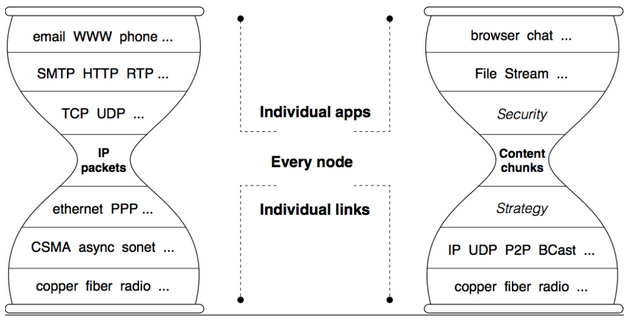
\includegraphics[scale=0.55]{./resources/figures/3_hourglass.png}
 %\caption{this is a test}
 \end{center}

%{\begin{figure}[t] \centering \includegraphics[width=#1cm]{resources/figures/#3.png} \caption{#2.} \label{fig:#3} \end{figure}}


} 

\item{
\textit{امنیت}
 یکی از ملزومات طراحی هر معماری‌ای است. امنیت در شبکه‌های امروزی، مسئله‌ای است که بعد از طراحی معماری به آن پرداخته شده است و در واقع در لایه‌های بالاتر و پایین‌تر از لایه شبکه به مسئله امنیت پرداخته شده و در محیط خطرناک اینترنت امروزی، امنیت مورد نیاز را تامین نمی‌کند. امنیت در شبکه‌های NDN یک مسئله پایه‌ای است و برخلاف شبکه‌های IP در همان لایه شبکه به آن پرداخته شده است و با امضا کردن محتوای بسته‌های داده این امنیت را در حد خوبی فراهم کرده است. 

}

\item{
\textit{روش انتها به انتها}
 که در شبکه‌های امروزی وجود دارد امکان مقابله در صورت بروز مشکل در شبکه  را فراهم می‌کند. اگر از روش انتها به انتها استفاده کنیم، در صورت از کار افتادن یکی از پیوندهای موجود در شبکه، از‌آنجایی که فقط به مقصد رسیدن بسته مهم است، مسیریاب می‌تواند بسته را از یک مسیر دیگر بفرستد و بسته در نهایت به مقصد خود می‌رسد ولی در صورتی که اگر از روش نقطه به نقطه استفاده شده باشد، در صورت بروز چنین رخدادی، بسته در میانه‌ی راه رها می‌شود. این رویه در شبکه‌های NDN هم وجود دارد. 
}

\item{
\textit{ترافیک شبکه}
باید به نحوی باشد که بتواند خودش را با تغییرات تطبیق دهد. جریان معتدل داده‌ها در داخل شبکه برای داشتن یک شبکه پایدار ضروری است. در سیستم مبتنی بر IP ، چون امکان به وجود آمدن حلقه در رسیدن بسته‌ها به مقصد وجود دارد، پروتکل‌های لایه انتقال هستند که در مقابل رویداد چنین وقایعی ارتقا داده شده‌اند. ولی در شبکه‌‌های NDN، در همان لایه شبکه مکانیزمی برای مقابله با به وجود آمدن حلقه در نظر گرفته شده است. 
}
\item{
\textit{جدا بودن دامنه مسیریابی و ارسال}
یکی از مسائلی است که ثابت شده برای توسعه اینترنت امری ضروری است. فایده این کار این است که سیستم ارسال می‌تواند به کار خود ادامه دهد درحالیکه سیستم مسیریابی به صورت مستقل خودش را با تغییرات شبکه تطبیق می‌دهد.  معماری حاکم بر NDN هم همین رویه را پیش‌رو گرفته و امکان مستقل کار کردن این دو دامنه را فراهم کرده است. 
}

\item{
\textit{ معماری باید انتخاب کاربر و رقابت را در مواقع امکان‌پذیر فراهم کند }
هرچند که این فاکتور، در طراحی معماری اصلی اینترنت جایگاهی نداشته است، ولی گسترش شبکه‌ها این قضیه را اثبات کرده است که معماری نباید نقش خنثی‌ای داشته باشد. معماری NDN تلاش آگاهانه‌ای در جهت قدرتمند کردن کاربران نهایی و همچنین به وجود آمدن رقابت کرده است. 
}

\end{itemize}

\section{معماری NDN}
مشابه شبکه‌های مبتنی بر IP، محوریت معماری شبکه‌های NDN  نیز همان میانه ساعت شنی ذکر شده در قسمت قبل است. ولی در این شبکه‌ها از داده‌‌های نام‌گذاری شده به جای آدرس‌های IP استفاده می‌‌شود. این تغییر علی‌رغم سادگی‌اش، موجب به وجود آمدن تفاوت‌های زیادی بین عملکرد این شبکه‌ها در رساندن بسته‌ها با شبکه‌های پیشین که مبتنی بر IP بودند، شده است.  در این بخش ابتدا یک توضیح مختصر راجع به مفاهیم کلی در شبکه‌های NDN داده می‌شود و سپس راجع به هر عنصر و هم‌چنین نقش آن در معماری کلی به تفضیل صحبت می‌شود. \\

\begin{center}
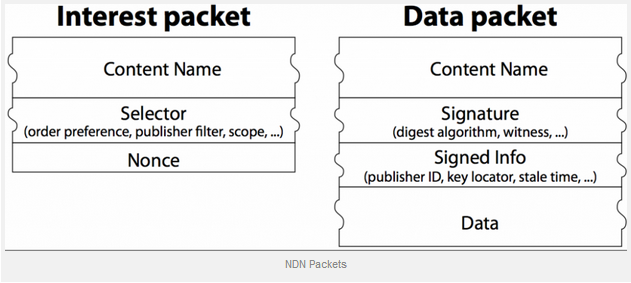
\includegraphics[scale=0.75]{./resources/figures/3_NDNpackets.png}
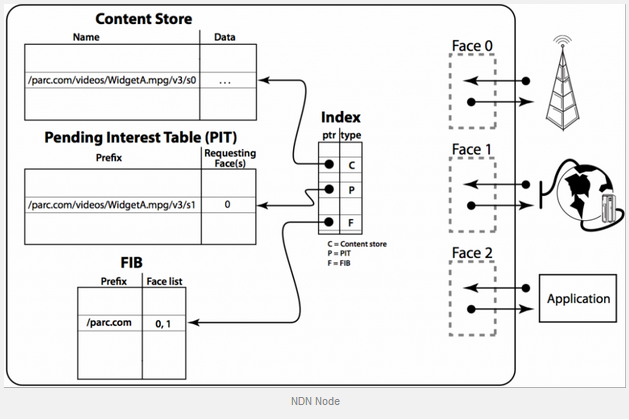
\includegraphics[scale=0.75]{./resources/figures/3_NDNnode.png}
\end{center}

ارتباطات در شبکه‌های NDN بر پایه درخواست یک مشتری آغاز می‌شود. مشتری برای اینکه به داده‌ای دسترسی پیدا کند، یک بسته از نوع درخواست می‌فرستد که شامل یک نام است که ماهیت داده مورد نظر را مشخص می‌کند (‌شکل ۲ )‌. مسیریاب واسطی که این بسته از آن رسیده است را به خاطر می‌سپارد و بعد این بسته را بر پایه داده‌های \textbf{جدول اطلاعات ارسال}  بر روی واسط درست ارسال می‌کند. 



\subsection{اسامی}
\subsection{امنیت داده‌محور}
\subsection{مسیریابی و ارسال}
\subsection{ذخیره‌سازی}
\subsection{جدول درخواست‌های معلق}
\subsection{انتقال}